\chapter{Drupal theming}

In this chapter we are going to learn how to change the look of our site. First we will learn how to change the basic theme settings. Next you will learn how to install a custom theme. The last part of this chapter explains how to extend a theme and add your own html and css.

\section{Theme basics}

\subsection{Changing the theme settings}

To view the settings of your current theme (Bartik) go to \textbf{Appearance $\rightarrow$ Settings}. On his page you can see a tab for each of the enabled themes (Figure \ref{fig:theme_settings_enabled_themes}).

\begin{figure}[H]
	\centering
	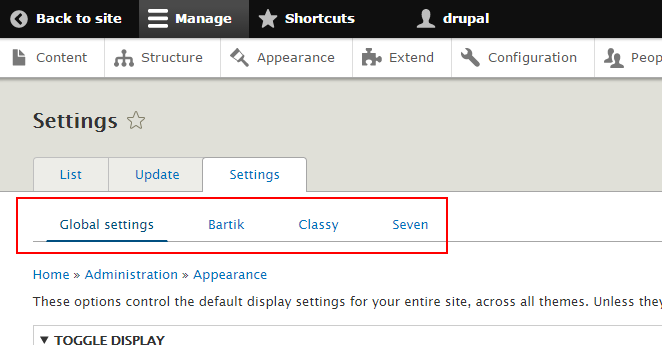
\includegraphics[width=\textwidth]{chapter10/theme_settings_enabled_themes}
	\caption{Theme settings, overview enabled themes.}
	\label{fig:theme_settings_enabled_themes}
\end{figure}

Some themes will come with more settings, such as colour options. Compare the themes you have enabled. Many theme specific settings are very similar to the global settings. When you change settings per theme, they will override the Global settings for that theme. Some of the more interesting themes will offer much more functionality. The default Bartik theme implements functionality from the Colour module, play around with them a little. The Colour module can, but does not have to be implemented in a theme, so not
every theme will offer this functionality.

\begin{figure}[H]
	\centering
	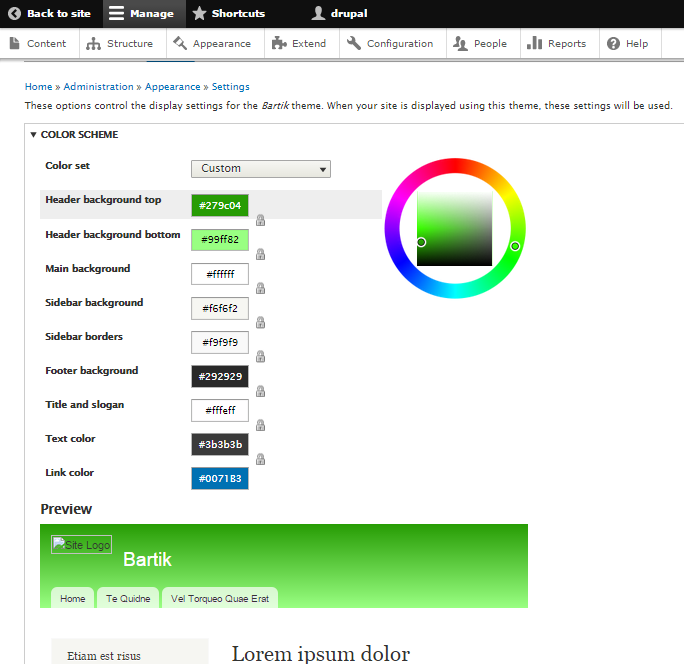
\includegraphics[width=\textwidth]{chapter10/bartik_color_settings}
	\caption{Changing the Bartik color settings.}
	\label{fig:bartik_color_settings}
\end{figure}

Notice in figure \ref{fig:bartik_color_settings} the logo image is not displayed. This is because we are using a custom logo image.

\subsection{Installing a new theme}

In Drupal there are several ways to install a theme. The fist option is to go to \textbf{Appearance $\rightarrow$ Install new theme}. 

\begin{figure}[H]
	\centering
	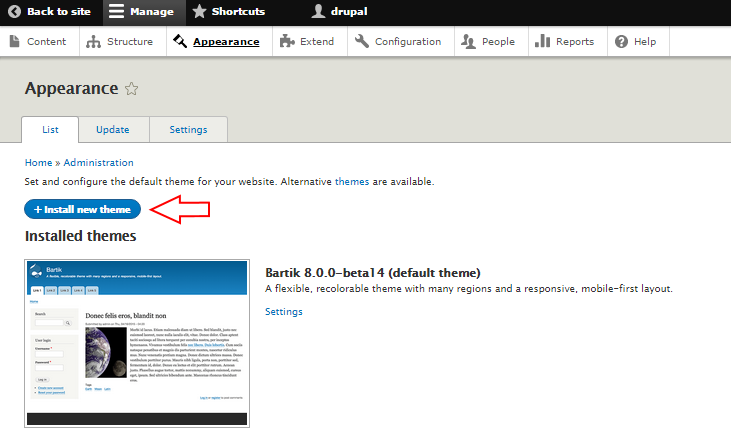
\includegraphics[width=\textwidth]{chapter10/install_new_theme_button}
	\caption{Click the button to install a new theme.}
	\label{fig:install_new_theme_button}
\end{figure}

This will take you to a page where you can either install from a URL, or upload an archive from your local computer.

\begin{figure}[H]
	\centering
	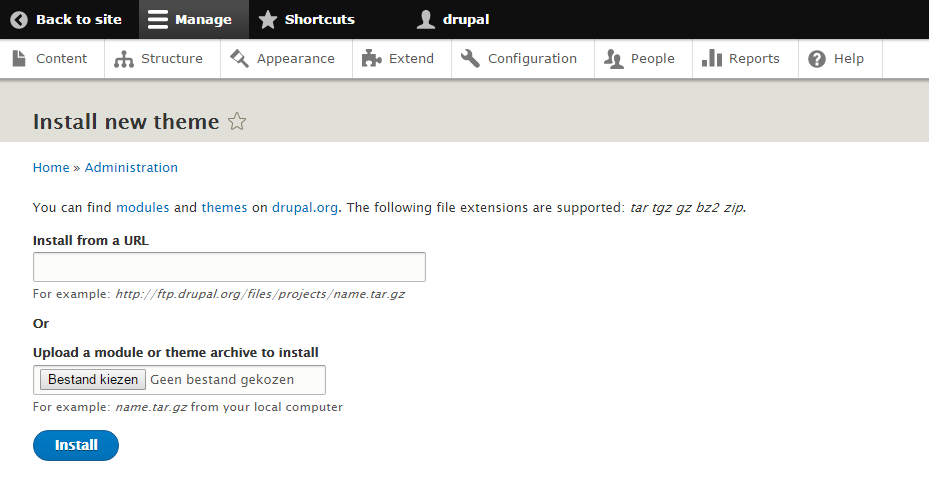
\includegraphics[width=\textwidth]{chapter10/install_new_theme_page}
	\caption{On this page you can choose to install a theme by copying the url from the location where the theme is hosted or uploading the theme from your local computer.}
	\label{fig:install_new_theme_page}
\end{figure}

Either way, you will have to visit the theme project page at \url{https://drupal.org/project/theme_name} and find the file URL for the archive, or just download it, which takes us to option number two.\\

The second way to install a new theme downloading it, unpacking it and placing it in the appropriate folder, which is \url{/themes} (Figure \ref{fig:theme_install_location}). 

\begin{figure}[H]
	\centering
	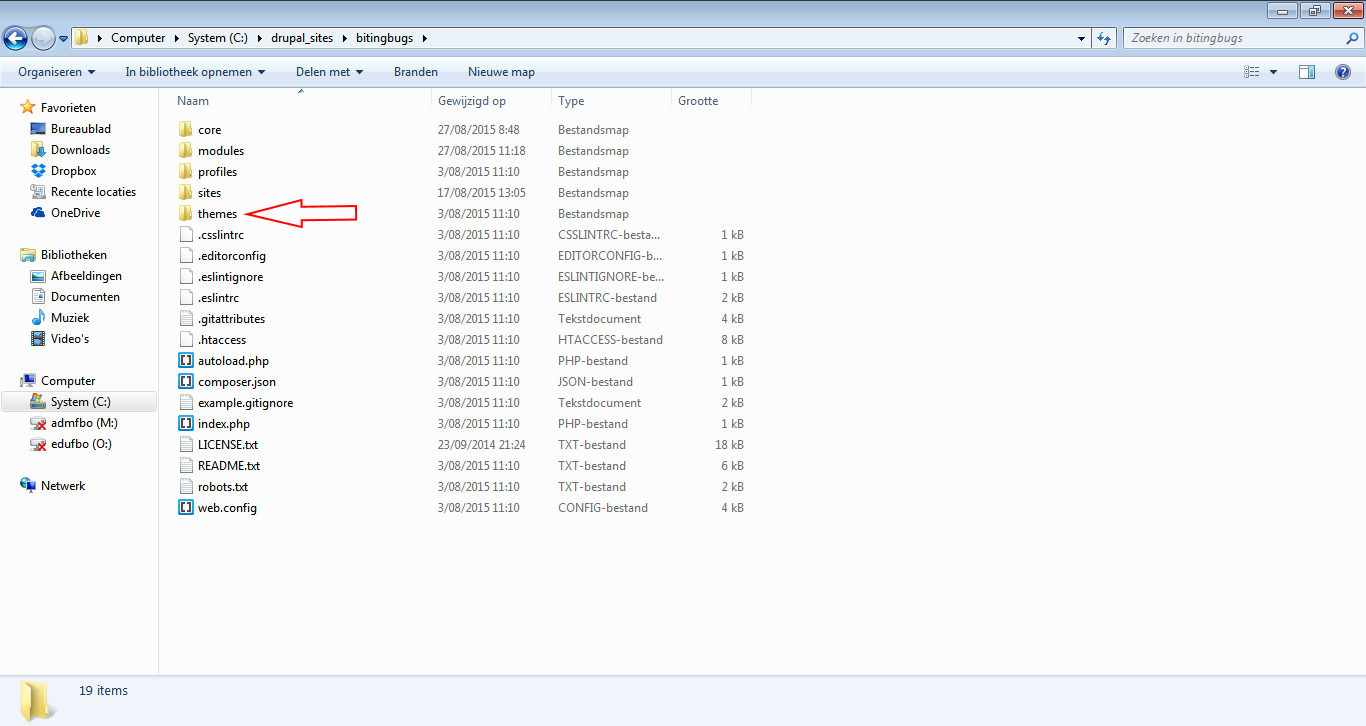
\includegraphics[width=\textwidth]{chapter10/theme_install_location}
	\caption{Theme install location.}
	\label{fig:theme_install_location}
\end{figure}

The third and quickest way to install a theme is through the Drush command line tool. Using Drush we have to type the following two commands:

\begin{lstlisting}[language=bash]
drush dl theme_name
drush en theme_name
\end{lstlisting}

The theme\_name, should be the machine name. This can be found in the URL of the project page on drupal.org, it is the word after project/. For example in \url{www.drupal.org/project/bartik} the machine name is \textbf{bartik}.

Drupal 8 has all core code and themes under a directory named /core. For contributed and custom themes drupal uses the /themes folder that lives on the same level as the /core folder. For people having experience with drupal 7 themes, these are the 2 most apparent changes when we look at a theme folder:
\begin{itemize}
	\item The *.infofile changes to *.info.yml.
	\item The *.tpl.phpfiles change to *.html.twig.
\end{itemize}

The README.txt file in the \url{/themes} directory says the following:\\

\textit{"Place downloaded and custom themes that modify your site's appearance in this directory to ensure clean separation from Drupal core and to facilitate safe, self-contained code updates. Contributed themes from the Drupal community may be downloaded at \url{http://drupal.org/project/themes}.	It is safe to organize themes into subdirectories and is recommended to use	Drupal's sub­theme functionality to ensure easy maintenance and upgrades. In multisite configuration, themes found in this directory are available to all sites. In addition to this directory, shared common themes may also be kept in the \url{sites/all/themes} directory and will take precedence over themes in this directory. Alternatively, the \url{sites/your_site_name/themes} directory pattern may be used to restrict themes to a specific site instance. Refer to the "Appearance" section of the README.txt in the Drupal root directory for further information on theming."
}

\section{Theme structure and subtheming}

\subsection{Creating your own theme}

To create a new theme navigate to your site \url{/themes} folder. For me this is the \url{C:\drupal_sites\bitingbugs\themes} folder. There we will create a new folder for our theme named \textbf{my\_new\_theme}. Inside the new folder we need a file to describe our theme. Drupal requires this file to be named: \textbf{[theme name].info.yml}. So in our case we create a file named \textbf{my\_new\_theme.info.yml}.

A \url{.yml} file is used for the YAML file type. YAML stands for YAML Ain't Markup Language. It is called this way because it strives to be as human readable as possible. Figure \ref{fig:yaml_file_example} shows an example of a YAML file. As you can see YAML files look very simple because they use whitespace to structure the content. 

\begin{figure}[H]
	\centering
	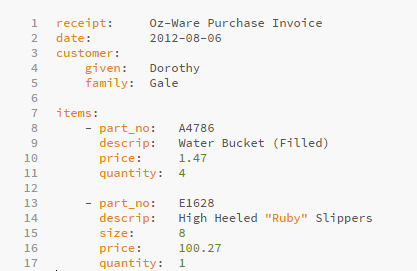
\includegraphics[width=\textwidth]{chapter10/yaml_file_example}
	\caption{An example of a basic YAML file.}
	\label{fig:yaml_file_example}
\end{figure}

The \url{.info.yml} file has four required keys (figure \ref{fig:info_yml_req_keys}):
\begin{description}
	\item[Name:] The human readable name will appear on the Appearance page, where you can activate your theme.
	\item[Type:] The type key indicates the type of extension, e.g. module, theme or profile. For themes this should always be set to "theme".
	\item[Description:] The description is also displayed on the Appearance page.
	\item[Core:] The core key specifies the version of Drupal core that your theme is compatible with.
\end{description}

\begin{figure}[H]
	\centering
	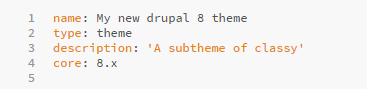
\includegraphics[width=\textwidth]{chapter10/info_yml_req_keys}
	\caption{Required info file keys.}
	\label{fig:info_yml_req_keys}
\end{figure}

Next to the required keys you can also add some other properties:

\begin{description}
	\item[Package:] The package key allows you to group themes together on the Appearance page.
	\item[Base theme:] : The theme can inherit the resources from another theme by defining it as a base theme.
	\item[Version:] For modules hosted on \url{drupal.org}, the version number will be filled in by the packaging script. You should not specify it manually, but leave out the version line entirely.
	\item[Screenshot:] With the screenshot key you define a screenshot that is shown on the	Appearance page. If you do not define this key then Drupal will look for a file named \url{screenshot.png} in the theme folder to display.
	\item[Libraries:] The libraries key can be used to add asset libraries — which can contain both CSS and JS assets — to all pages where the theme is active.
	\item[Stylesheet­remove:] The stylesheets­remove key removes a link to a stylesheet added by another theme or module. The full path to CSS file should be provided (instead of just the filename), to accommodate cases where more than one file with the same name exists. In cases where a Drupal core asset is being removed (for example, a CSS file in jQuery UI) the full file path is needed. In cases where the file is part of a library that belongs to a module or theme, a token can be used. Note that when using the token it needs to be quoted because @ is a reserved indicator in YAML.
	\item[Regions:] Regions are declared as children of the regions key. You are required to have a content region.

\end{description}
